

\chapter{Konstruktion und Design}
\label{chap:konstruktion}


\section{Strukturelles Design des autonomen Segelschiffs}
\subsection{Wahl der Applikation}
Computer Aided Design (CAD) ist eine Form des technischen Zeichens, welches einem ermöglicht Modelle in Drei dimensionalen Raum zu gestalten. Im Vergleich zum konventionellem 3D Modelling. welches vorallem aus Bereichen wie CGI und Animation bekannt ist, arbeitet man mit CAD mit festen Grössen und Masseinheiten anstatt dem verschieben und Bewegen von Netzen (Mesh). Somit lässt ist es verhältnissmässig einfach Technische Zeichnungen anzufertigen. Es gilt als eines der Wichtigsten Werkzeuge zur Planung von Maschienen und Geräten da sie so einfacher Vorstellbar sind und der Materialbedarf geplant werden kann. Die Konstruktion dieses Projekt beginnt mit dem erlernen von den Programmen Autodesk Inventor und Autodesk Fusion 360. 
Beide Programme verfolgen einen ähnlichen Ansatz und sind ähnlich Aufgebaut. Im Vergleich zu Inventor ist Fusion deutlich nutzerfreundlicher und ermöglicht es Projekte über eine Cloud einfacher zu speichern und von Unterwegs zu Bearbeiten. Die Programme von Autodesk wurden gewählt, da diese für den Persönlichen oder Bildungsgebrauch kostenlos sind. Open Source Programme wie FreeCAD wurden nicht gewählt, da diese weniger Intuitiv zum lernen sind und meist über weniger Funktionen verfügen. Programme welche als deutlich Leistungsstarker gelten wie NX Siemens oder Solidworks sind aufgrund der Lizensierungskosten für dieses Projekt nicht in Frage gekommen. 


\subsection{Vergleich von verschiedenen Segelboot Typen}

\subsubsection{Rumpftypen}
Die erste und einfachste Unterscheidung von verschiedenen Segelboot Typen ist die Anzahl an Rümpfen. Wenn man sich ein Segelboot vorstellt, denkt man meist an ein "mono hull". Jedoch gibt es auch den "double hull" oder man Kategorisiert sie als "multi hull" welche vorallem aus der Welt der Kathamarane und Trimarane bekannt sind.\\
Der Rumpf an sich kann jedoch auch innerhalb von einer von diesen Kategorien komplett unterschiedlich geformt sein. 
%
\subsubsection{Segeltypen}

\subsubsection{Kieltypen}

\subsubsection{Rudertypen}

\section{Prozess der Konstruktion des Rumpfes}
\subsection{Statik}
Wie bereits erwähnt wurde das Schiff so konstruiert, dass es mögliche, starke Krafteinwirkungen standhalten könnte. Daher wurde auf die Interne Kraftverteilung stark geachtet.
\subsubsection{Rippenmuster und dessen Besfestigung}
Ein Rippenmuster, wie es bei Holzbooten üblich ist, wurde verwendet um die Form zu bestimmen. Diese wurden mit einem Geringen Abstand von (Länge einfügen) Plaziert um auch bei seitlichen Krafteinwirkungen genügend Strukturelle stütze zu sein.

\begin{figure}[H]
  \centering
  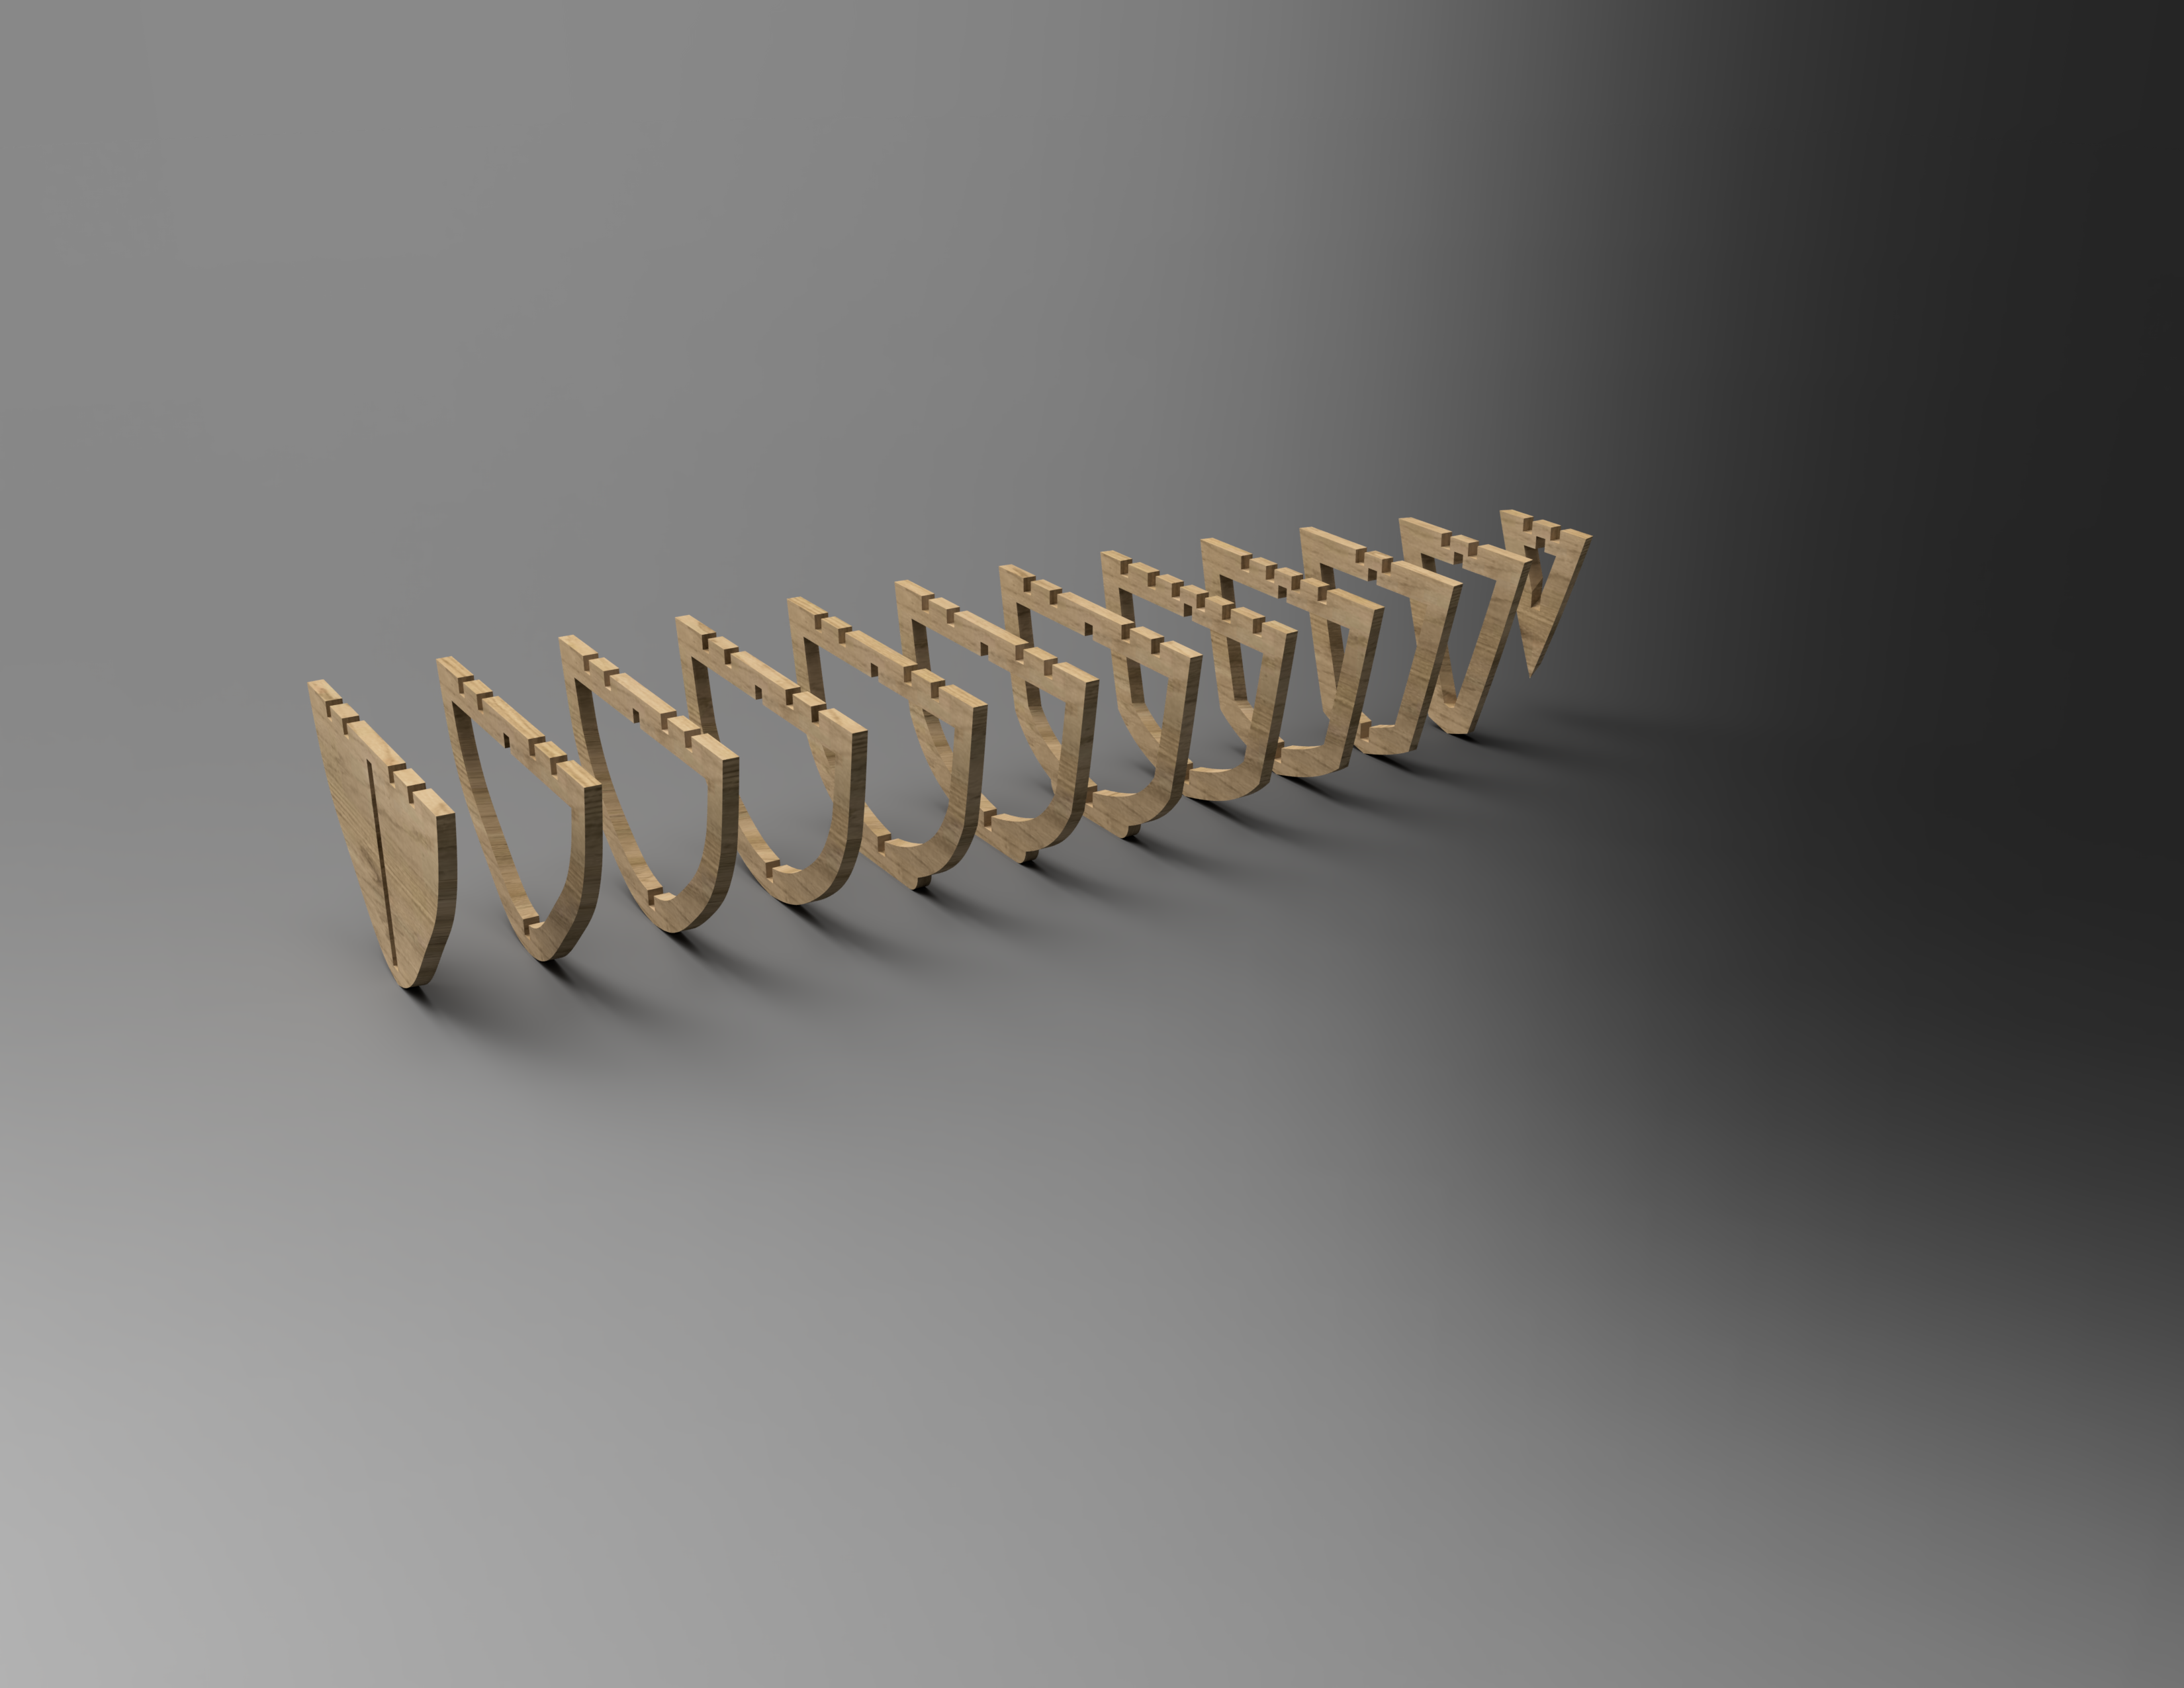
\includegraphics[width=\textwidth]{assets/rippenv1.png}
  \caption{Render einer ersten Version des Rippenmusters (nicht Final) }
  \label{fig:rippenv1}
\end{figure}


\section{Materialauswahl und -begründung }
\subsection{Holz}
Die strukturell Tragenden Elemente sind Hauptsächlich aus Holz gebaut. Dies hat den entscheidenden Vorteil der einfachen Verarbeitung. Ebenso hat Holz den Vorteil, dass es an sich schon schwimmt da es weniger Dicht als Wasser ist. Konkret werden zwei Holzarten verwedet. Zum einen Tannenholz und zum anderen Balasaholz. Das Tannenleimholz wird mit einer Stärke von 18mm verbaut und ist das kostengünstigste Holz was in dieser Kategorie im Baumarkt zu finden ist.
Alternativen zu Holz wären diverse Kunststoffe wie PLA, ABS, PETG, ect. welches durch 3D Druck geformt werden können. Jedoch wären die Kosten bei dieser Methode deutlich höher und eine gleiche Stabilität wie bei Holz zu erreichen wäre eine Herausforderung.
Ebenfalls möglich sind Rippenelemente aus Metallen, wie zum Beispiel Aluminium. Die Materialkosten sind bei Metallen jedoch weitaus höher und die Bearbeitung um ein vielfaches Komplizierter weshalb sich dagegen entschieden wurde.
\\
Für die Beplankung wurde sich für Balsaholz enschieden, da dies eines der Weit verbreitesten Materialien im Bereich des Modelbau ist. Mit einer geringen stärke von 1mm lässt es sich gut an die Form des Bootes anpassen.
% Balsaholz ABschnitt hinzufügen

\subsection{Fiberglas}
Für die äussere Hülle werden Fiberglasmatten verwendet. Diese sorgen für eine stabile Hülle und schützen das Boot zusätzlich vor seitlichen Zusammenstössen. Ebenfalls sorgen sie dafür, dass das Boot dicht ist und kein Wasser hineinfliesst. Alternativ hätte man das Boot lediglich mit Epoxidharz abdichten können. Dies hätte aber dazu geführt, dass das Boot um ein vielfaches weniger stabil wäre. 

\section{Segel und Sailflap}
Beim Design des Segels wurde viel von einer Bestehenden Arbeit übernommen. Diese hat sich mit der Entwicklung eines Segels für den Einsatz auf dem Baltischen Meer spezialisiert.



\section{Entwicklungsprozess des Kiels}
Der Entwicklungsprozess des Kiels ist aufgrund der geringen Literatur in diesem Bereich sehr aufwendig. \\ Die erste Frabstellung in diesem Bereich, ist ob es sich um ein Kiel oder ein Schwert handeln soll. Die Unterschiedung liegt grob darin, dass ein Kiel zusätzliches Gewicht trägt, um das Boot aufrechter zu halten und Schwerter lediglich den Wasserwiederstand. Kiele sind hauptsächlich aus der Welt der Jachten bekannt und Schwerter aus der Welt der Jollen. \\
Für dieses Boot wurde sich für ein Kiel entschieden, da es auf dem Boot keine möglichkeit gibt, Gewicht zu verschieben. Bei Jollen ist in der regel ein Segler auf dem Boot, welcher sehr viel mit seinem eigenen Körpergewicht steuert. Bei den meisten Jachten spielt das Körpergewicht der Segler keine oder nur eine untergeordnete Rolle.